\section{Theory}
Most dMRI approaches in the context of dMRI are applying it to generate
probabilistic tractographies out of deterministic tracking approaches. Such
approaches are reviewed in Section \ref{related}. 

Our first novel contribution is to determine the uncertainty caused by
measurement errors to the proposed models in a systematical way. Therefore, wild bootstrapping is used to create
noisy resamples out of the measurements. The resampled data is then processed
and the parameters of a Watson distribution are evaluated to measure the
uncertainty which is propagated through the dMRI pipeline. 

As a second contribution we introduce a novel model, which reduces the measurement
uncertainty by incorporating all bootstraps into a new bootstrap consensus model.

\subsection{Wild Bootstrapping}
To evaluate the impact of measurement errors we use wild bootstrapping. It
has been shown in many cases that it is well suited within the context of dMRI and
is a straight forward way to
resample the original measurement without redo the measurement process
\cite{Jones:2008}.

To create bootstrap samples the following process is applied. As a first step the model is fitted to the data. We obtain a fODF
$\hat{\mathcal{T}}$ and can calculate residual of Eq. (\ref{eq:sd-min}) 
\[ \hat{\varepsilon} = S - M\hat{\mathcal{T}} .\] 
A new bootstrap realization is calculated by 
\[ y^{*} = M\hat{\mathcal{T}}  + \hat{\varepsilon} v , \]
where $v$ denotes a random draw from the $n$ dimensional Rademacher distribution
\[ f \left( \mathbf{k} \right) \coloneqq  \begin{cases} \nicefrac{1}{2} \text{ if }
		\mathbf{k}_i=-1 \\
		\nicefrac{1}{2} \text{ if } \mathbf{k}_i=1 \\
		0 \text { otherwise } 
\end{cases} \text{ for } i \in \left\{ 1\dots n \right\} . \]
 Finally the model is fitted to the bootstrap realization. This process is repeated $m$
times to create a sample size of $m$ bootstraps.

For each sampled fODF we calculate the low-rank approximation of rank $3$
and with the obtained residuals also the selection and average model as it was
proposed by Gruen et al. \cite{Gruen:2021}.

\begin{figure*}[h]
	\centering
	\begin{subfigure}[b]{0.33\linewidth}
		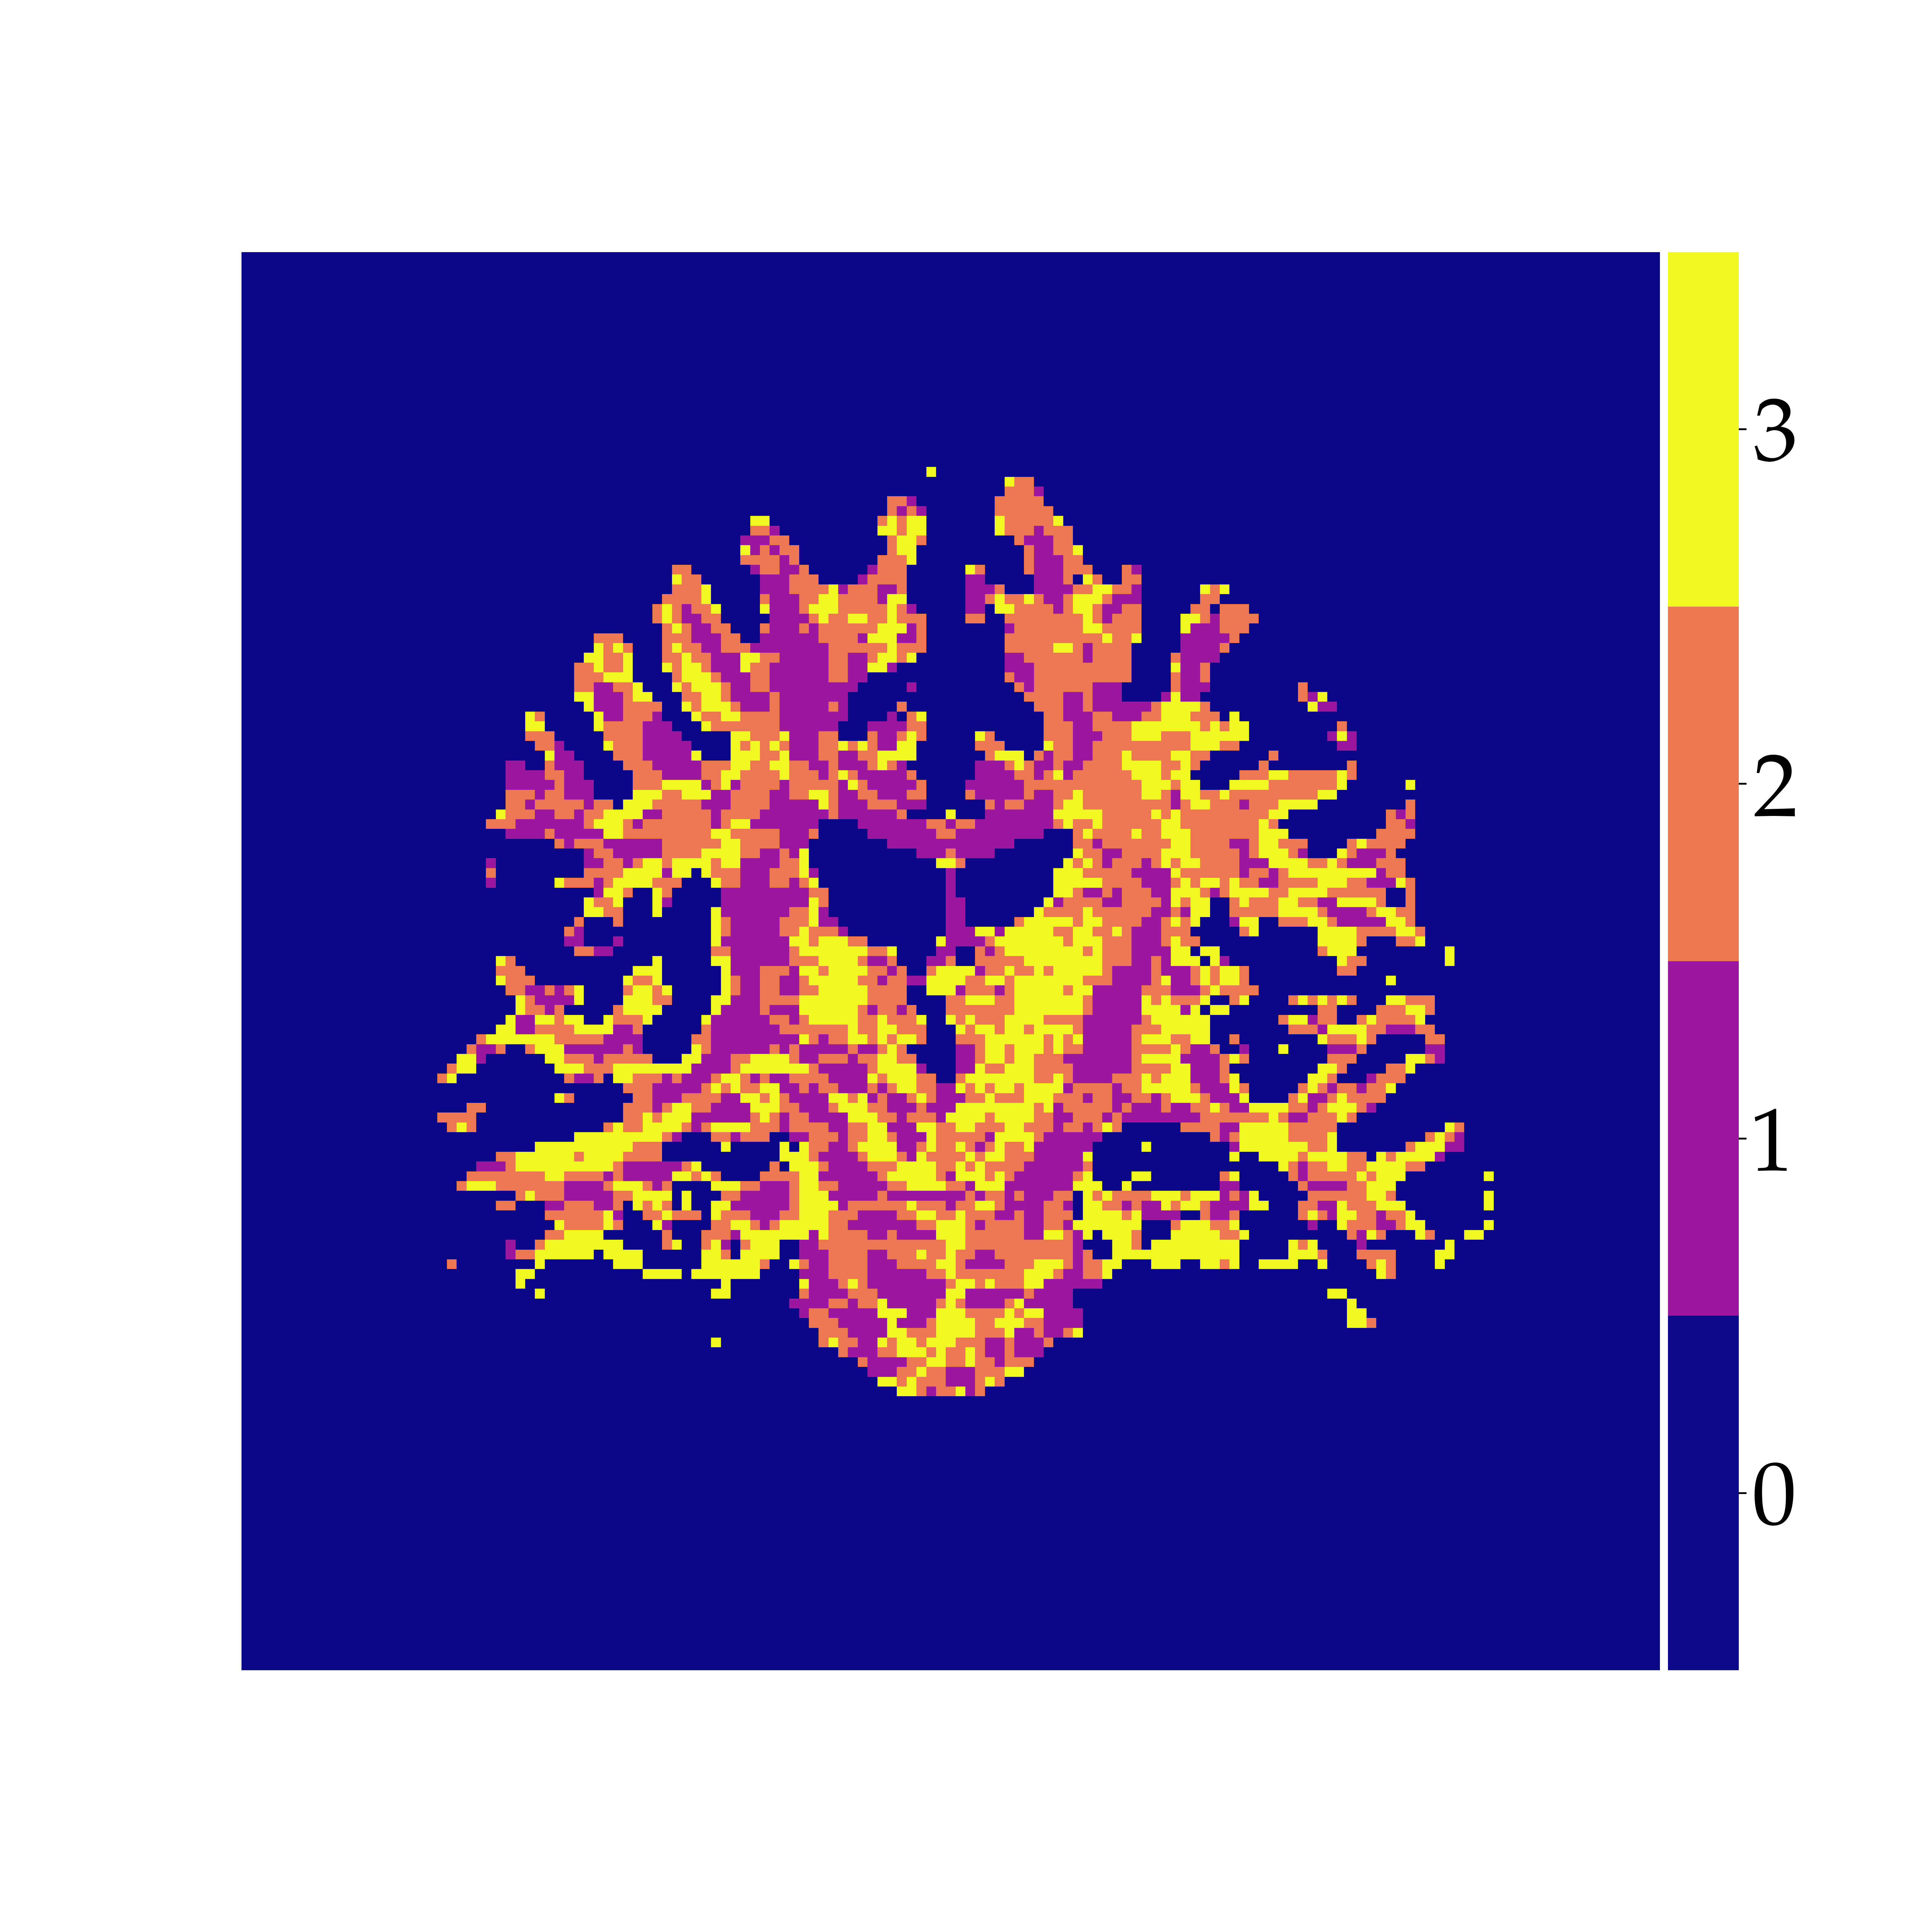
\includegraphics[width=\linewidth]{selected}
		\caption{The most likely number of fiber according to the
		selection model}
	\end{subfigure}
	\begin{subfigure}[b]{0.33\linewidth}
		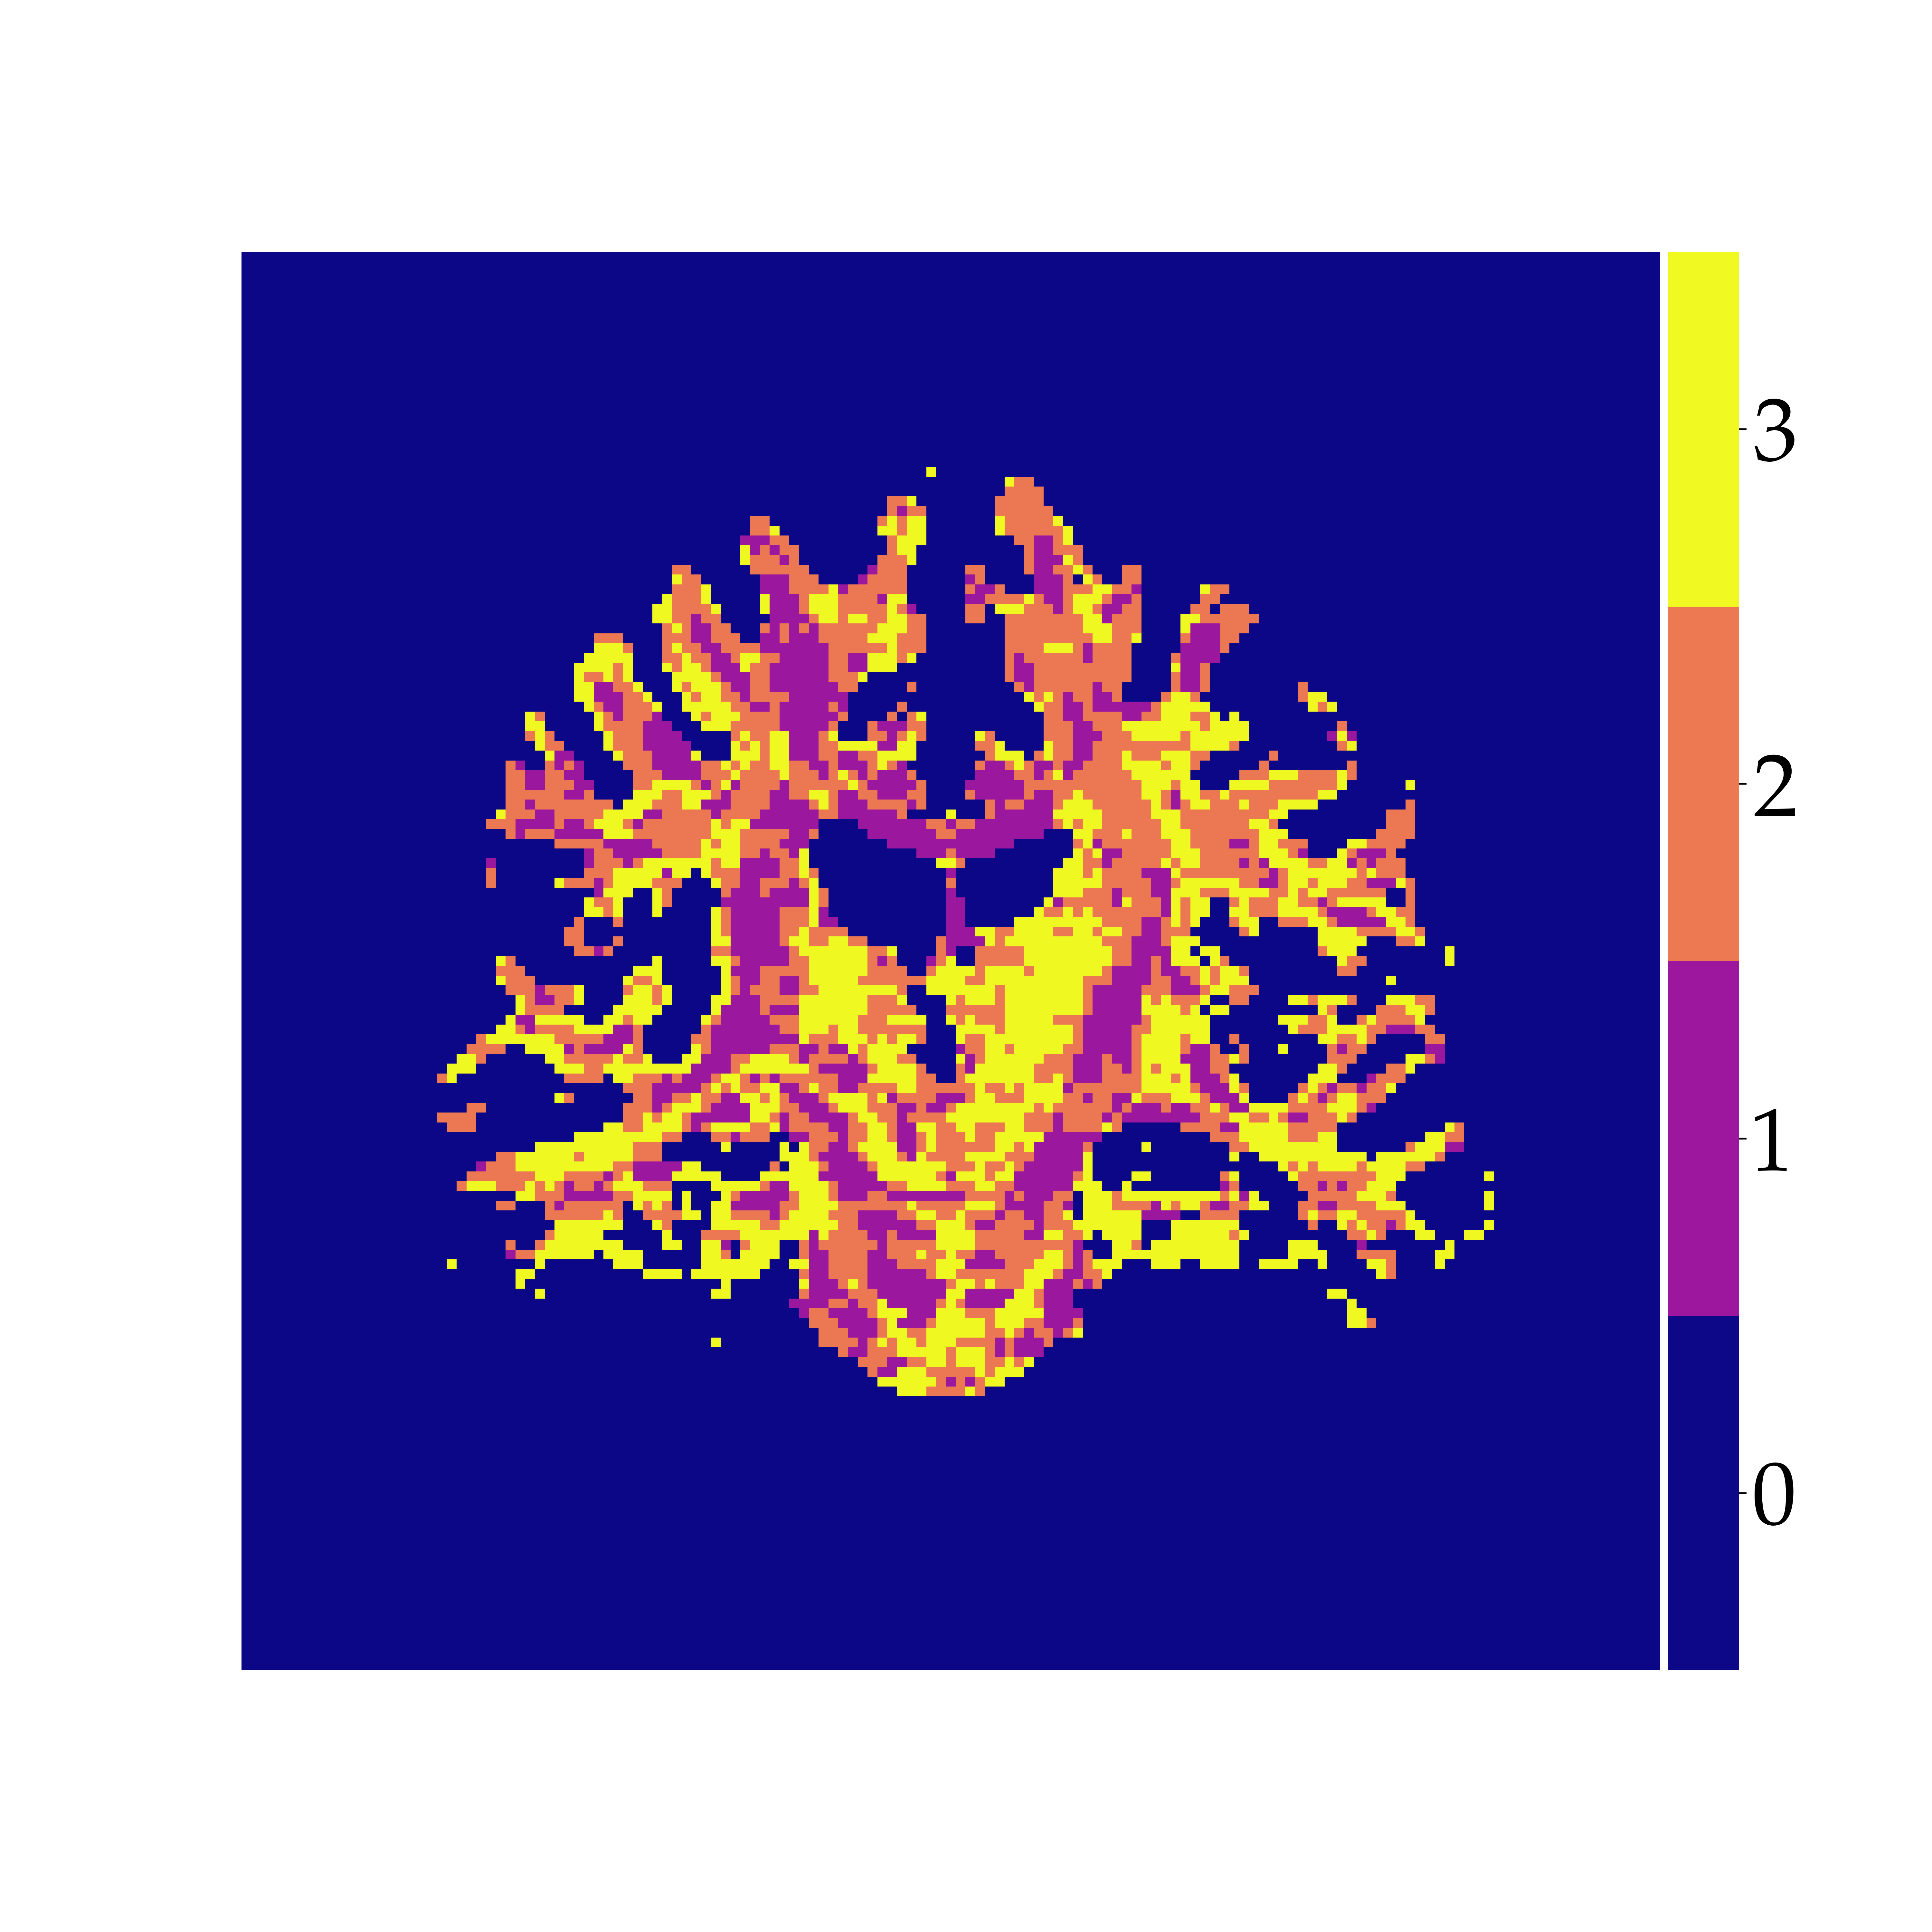
\includegraphics[width=\linewidth]{selected-bootstrap}
		\caption{The most like number of fibers over all bootstraps.
		$SSIM=0.77$}
\end{subfigure}  \\

	\begin{subfigure}[b]{0.33\linewidth}
		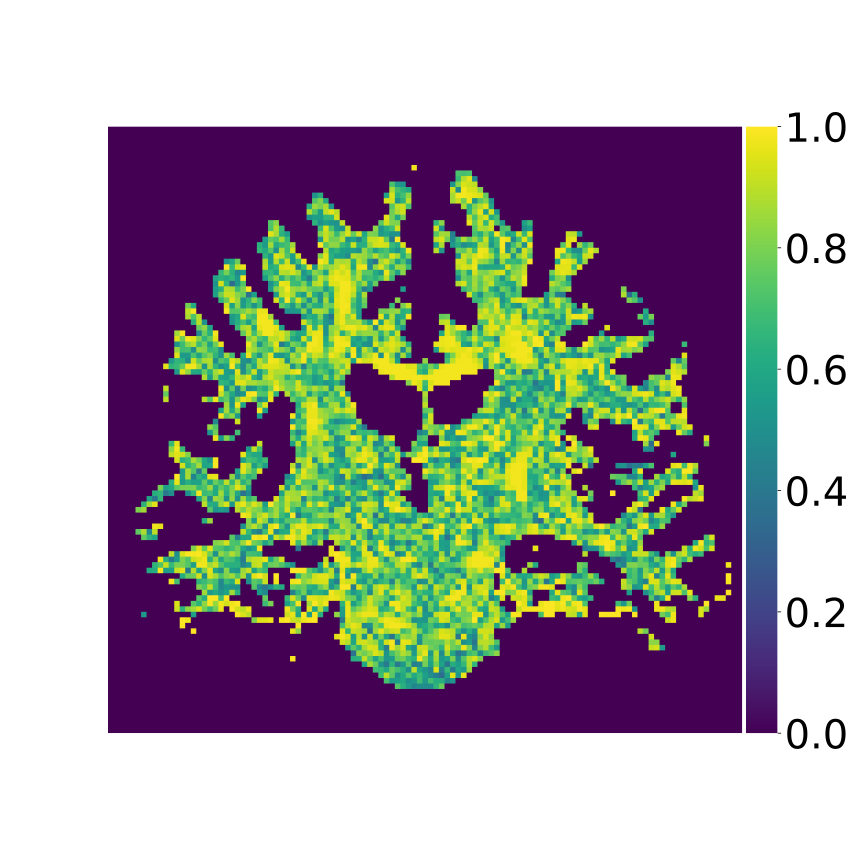
\includegraphics[width=\linewidth]{uncertainty}
		\caption{Certainty of the selected model.}
	\end{subfigure}
	\begin{subfigure}[b]{0.33\linewidth}
		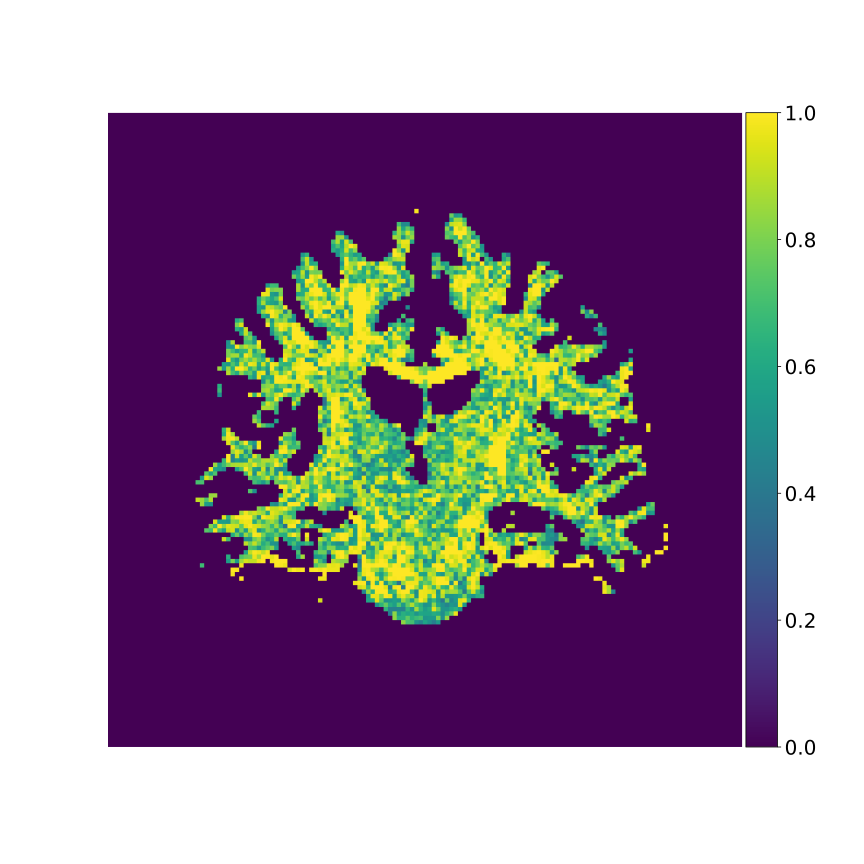
\includegraphics[width=\linewidth]{uncertainty-bootstrap}
		\caption{Number of bootstraps, which selected the most likely
		model over all bootstraps. $SSIM=0.67$}
	\end{subfigure}
	\caption{Comparison of model selection with and without bootstrapping.}
	\label{fig:selected-uncertainty}
\end{figure*}
As a first contribution we investigate the distribution of the selected ranks
over all bootstrap. Therefore, we have simulated 100 bootstraps and applied the
selection model to all of them. In Fig. \ref{fig:selected-uncertainty}, the most
likely model in the original data and the uncertainty of the selected model is
plotted in the left column. Further the generalization to the bootstrap model is
plotted within the right column. Here the most likely number of fibers is
calculated by selecting the model, which occurs most in bootstraps. The count of
occurrences can be interpreted as uncertainty, e.g. if the selection model takes
always the same model not mattering the bootstrap errors, it is very certain
that this model fits the data well.  
In most cases the selection model coincides with the most bootstrapping this
also get justified by a high SSIM of $0.77$ which is just calculated on the
image area, to avoid the influence of the similar background
\cite{wang2004image}.  Further the
bootstrapping has in general an high impact, which can be seen since the
selection model does not select always the same model within all the different
bootstraps.  



\subsection{Bootstrap Consensus Model}
Instead of using the bootstrap samples to produce a probability density map of
streamlines, we use it to reduce the measurement uncertainty by fusing the
information of all bootstraps into a new model. 
Therefore, the directions of all bootstraps get clustered to groups and the
group means are the new directions.

To build a consensus model we have to assign $n$ directions to $m$ groups on voxel
level. We initialize the process by setting the directions of the original model
as reference directions for the $m$ groups. Now each
direction is assigned to a group such that the sum of angles between group
reference and direction is minimized over all possible assignments to the
groups, i.e. we want to minimize the objective function 
\begin{align}
	T : \text{Sym} \left( r \right)^n & \mapsto \mathbb{R}_+ \nonumber \\
	Z & \rightarrow \sum \arccos | \langle \mathbf{v}_{Z\left( i
	\right)}, \mathbf{v}_i \rangle | ,  
\end{align} 
where $\text{Sym}\left( r \right)$ denotes the symmetric group and $\mathbf{v}$ denotes
the reference direction. To prevent wrong assignments if only one reference
direction is initialized we first assign the highest fiber count to the
groups and update the uninitialized reference directions with the assignments.
Note that this does not necessary lead to a global optimum, but is in most cases
close to the optimum. 

\begin{figure*}[t]
	\centering
	\begin{subfigure}[b]{0.33\linewidth}
		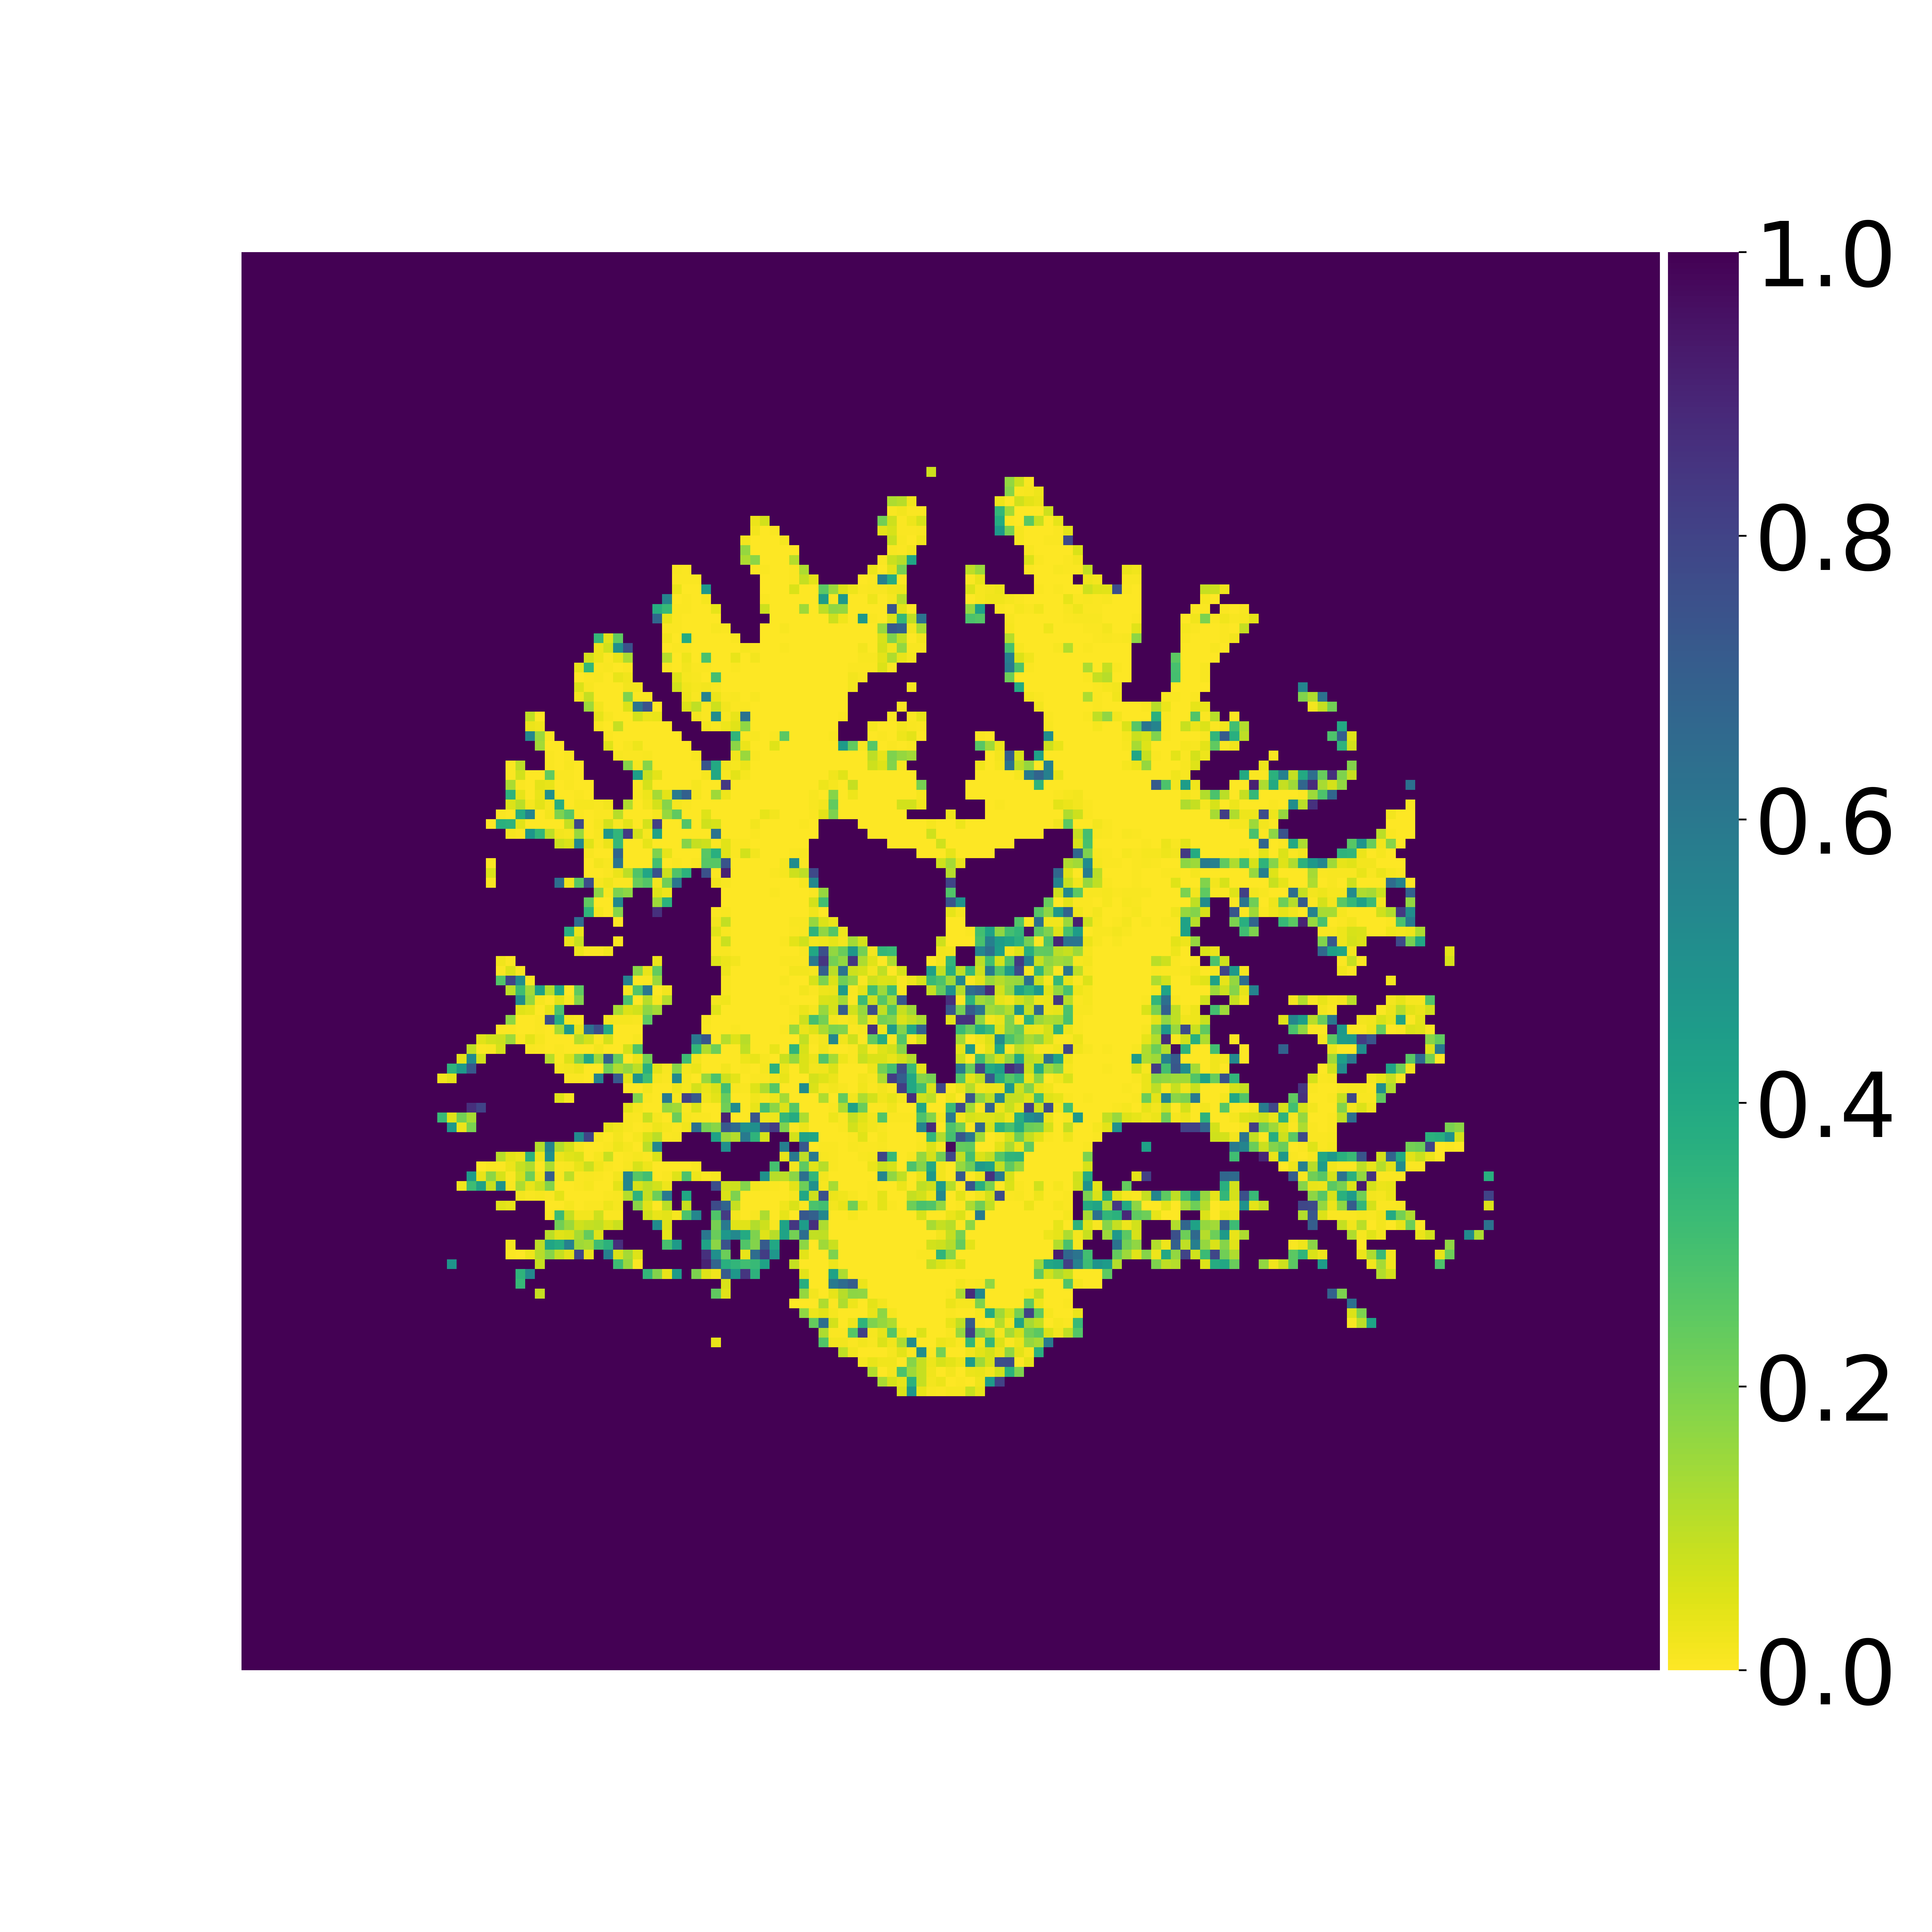
\includegraphics[width=\linewidth]{sel-bootstrap}
		\caption{Selection model}
	\end{subfigure}
	\begin{subfigure}[b]{0.33\linewidth}
		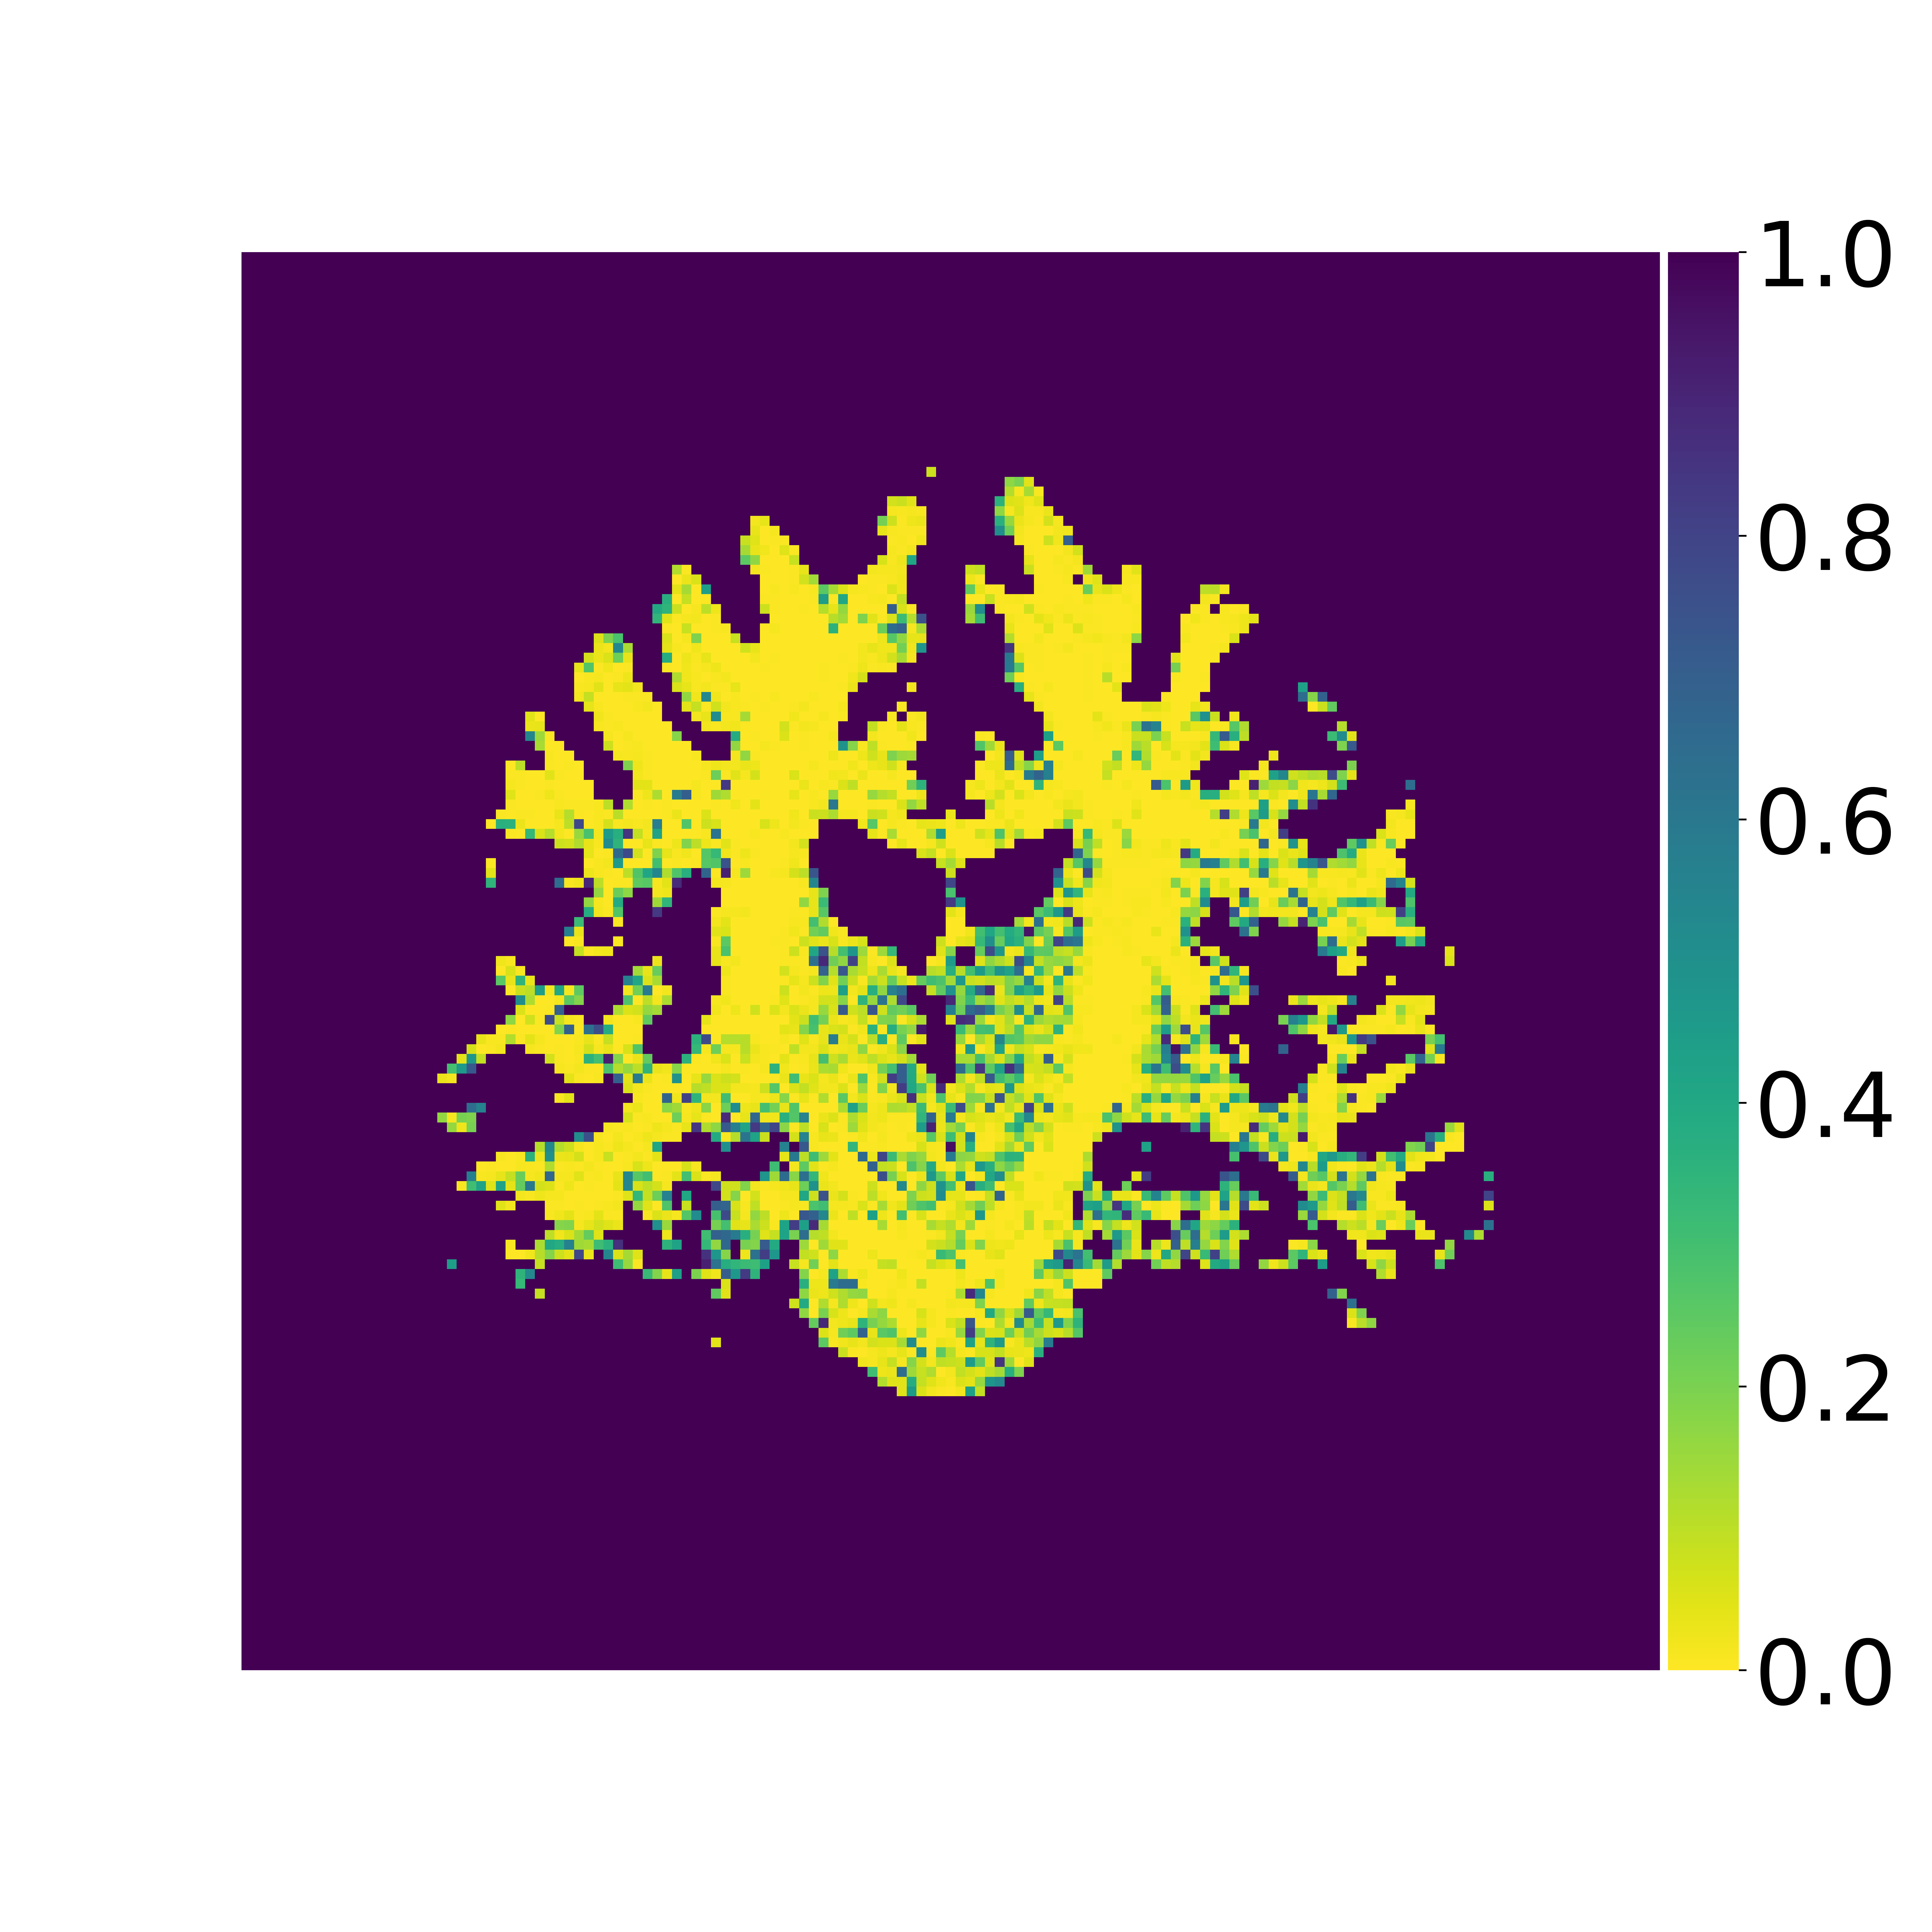
\includegraphics[width=\linewidth]{avg-bootstrap}
		\caption{Average model}
	\end{subfigure}
	\begin{subfigure}[b]{0.33\linewidth}
		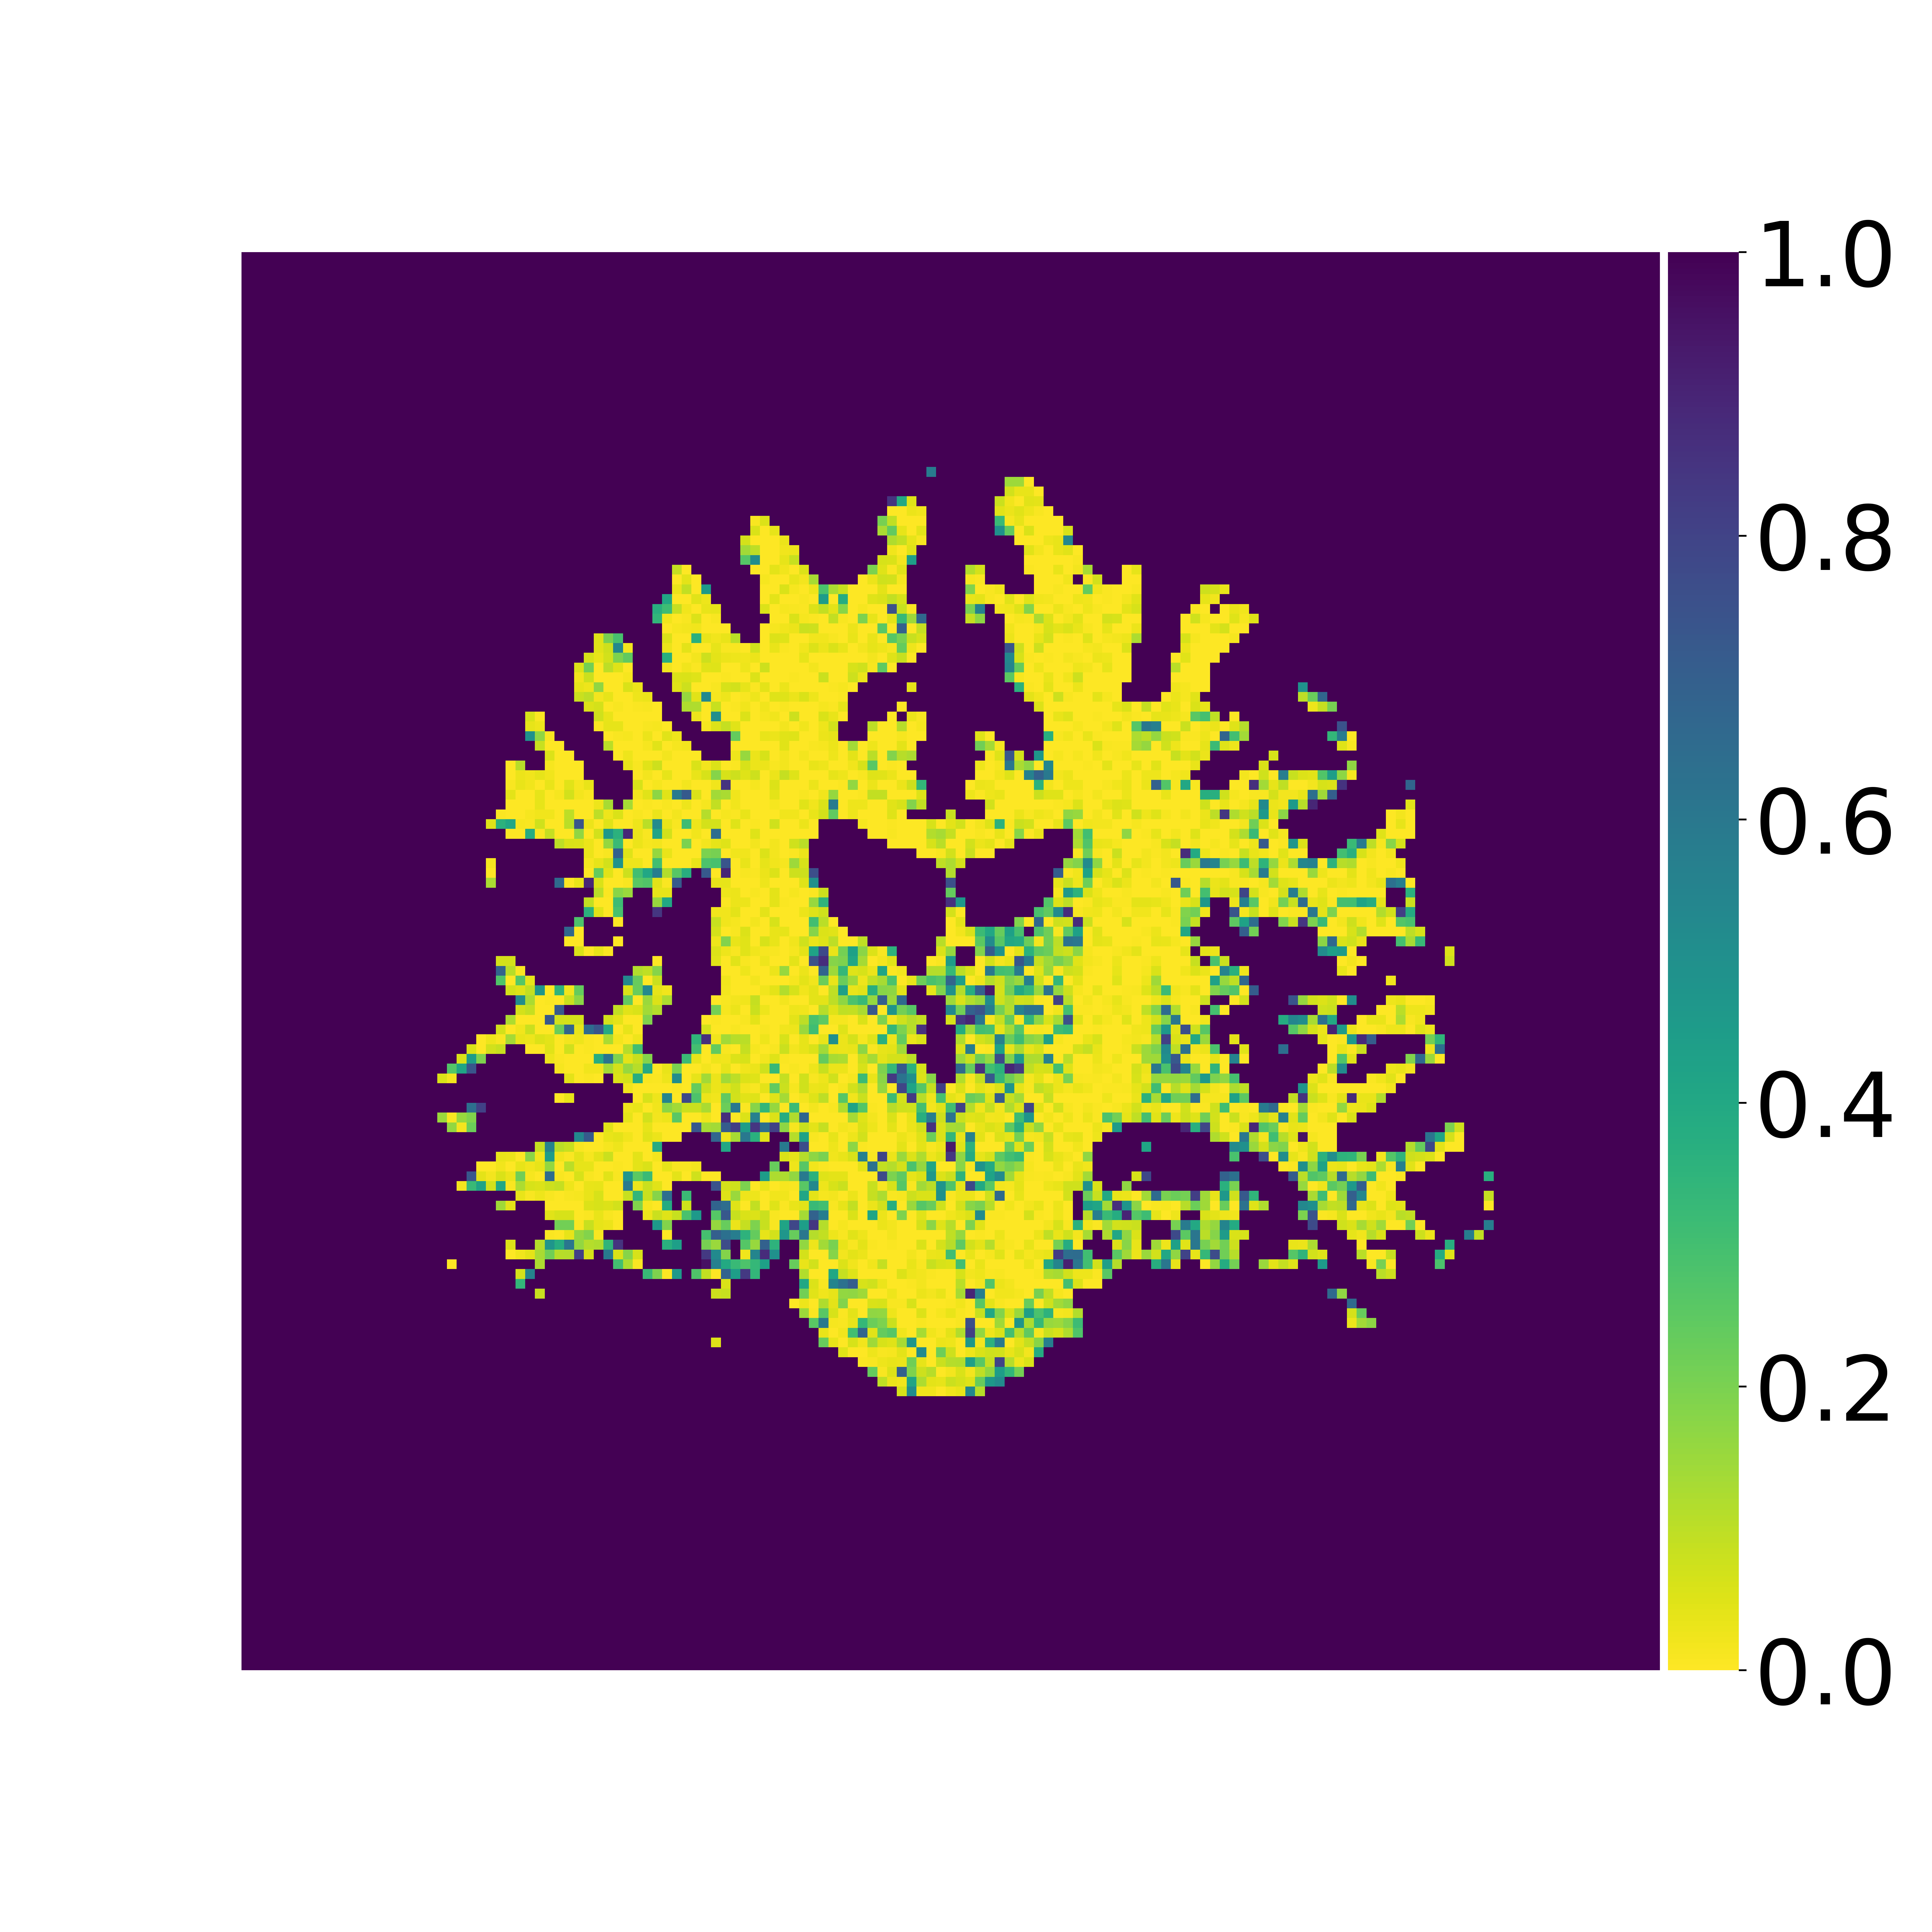
\includegraphics[width=\linewidth]{rank-bootstrap}
		\caption{Rank 3 model}
	\end{subfigure}
	\caption{Redefined orientation dispersion index calculated for the main
	direction of 100 bootstraps.}
	\label{fig:dispersion}
\end{figure*}

To get deeper insights into the impact of the bootstrapping we fit a Watson
distribution to the grouped directions.The Watson distribution is defined as  
\begin{align*}
	f : \mathbb{S}^2 & \longrightarrow  \mathbb{R}_+ \\
	\mathbf{x} & \longmapsto  M \left( \frac{1}{2}, \frac{3}{2} , \kappa
	\right)^{-1} \exp \left(  \kappa
	\left( \mathbf{\mu}^T \mathbf{x} \right)^2 
	\right) 	,  
\end{align*}
where $\kappa$ is the dispersion parameter, $\| \mathbf{\mu} \| = 1$ the
mean direction and $M$ be the confluent hypergeometric function. 

We use the Watson distribution because it has two main advantages. First of all it is antipodal symmetric,
which fits our model assumption of indistinguishable $\pm \mathbf{v}$
directions. Secondly, it is one of the easiest models for axial data and
introduces the dispersion parameter, which give us deeper insights into the
uncertainty within the groups. 

In Fig. \ref{fig:dispersion} we have visualized the redefined orientation dispersion index
\cite{dispersionParameter}  
\[ OD = \frac{2}{\pi} \arctan \left( \frac{1}{\kappa} \right) \] 
for the selection, average and rank 3 model. This score is more intuitive since
it maps the low dispersion to low values and vice versa. It is visible that the
selection model shows lower dispersion in large parts of the CC and CST tracts
compared to the average as well as the rank $3$ model. This is caused by the
ability of the selection model to select the rank $1$ model in this areas, which
is not as susceptible to noise as higher rank models. I.e. the selection model
reduces the impact of measurement noise without explicitly being build for
this. 
Therefore, we assume that the impact to the average and rank $3$ model is higher
than to the selection model. However, it will also have an impact to the
selection model, which is also susceptible to noise in higher rank areas. 

\begin{figure*}[t]
	\centering
	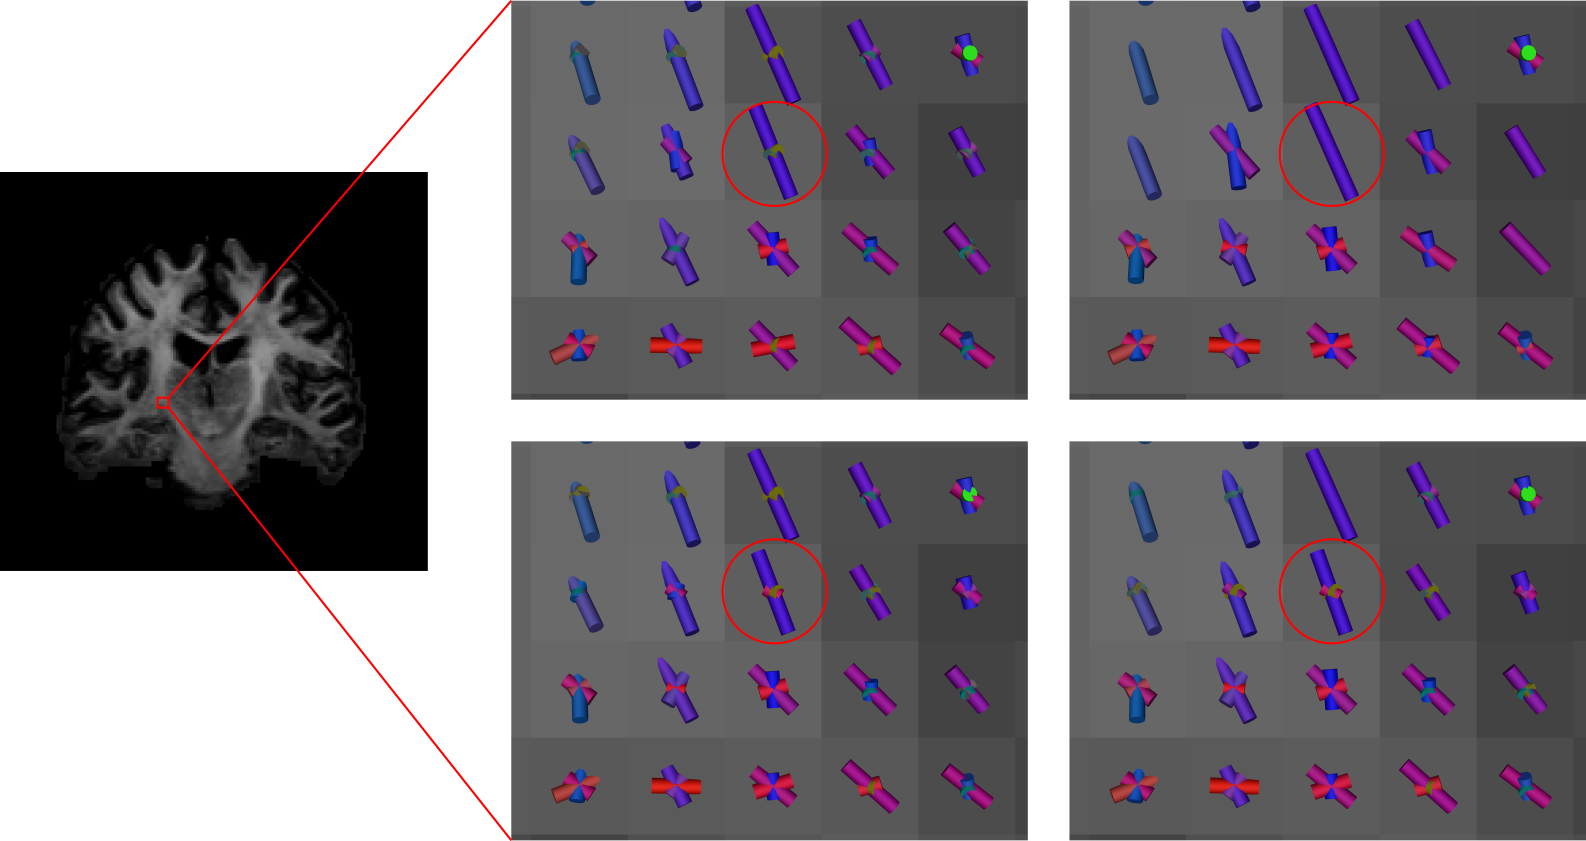
\includegraphics[width=\linewidth]{dir}
	\caption{Reconstructed fiber orientations of the different models, the
	red box in the left image denotes the position within the brain. Top row
shows models without consensus bootstrapping, bottom row with consensus
bootstrapping. From left to right: Averaging model, selection model, rank-$3$
model.}
	\label{fig:directions}
\end{figure*}

After having investigated the dispersion of the main direction it is also
important do understand the impact of the newly proposed model on the direction
fields which are plotted in Figure \ref{fig:directions}. 
The most obvious observation seems to be that the consensus bootstrap model generated
from the selection model has now in almost all voxel 3 fiber directions. But we
also see that the consensus model of the average and selection model coincide in
large parts. Interestingly also in voxels where the average model looks
differently than the selection model, compare the red marked 1. 
Since the difference between the main directions is hardly visible, we have
colored the background regarding the difference of the main direction. Here we
see that also within the rank $3$ vector field some changes are made. 

